%\documentclass[dvipdfmx]{beamer}
\documentclass{beamer}                   % lualatex の場合
\usepackage{mySld}
\begin{document}
\title[FATファイルシステム]
      {オペレーティングシステム\\第16章 FATファイルシステム}
\date{}
\begin{frame}
  \titlepage
  \centerline{\url{https://github.com/tctsigemura/OSTextBook}}
\end{frame}

%\section{}
%=========================================================================
%\begin{frame}
%  \frametitle{}
%\end{frame}

\section{FATファイルシステム}
%=========================================================================
\begin{frame}
  \frametitle{FATファイルシステム}
  \begin{itemize}
  \item 1980年代からPCのファイルシステムとして利用されてきた.
  \item 仕様が公開されているので様々なところで利用されている.
    \begin{itemize}
    \item USBメモリ,SDカード,その他メモリカード
    \item Windows,Linux,macOSはFATファイルシステムをサポート \\
      → 同じUSBメモリを使用してデータ交換が可能
    \item デジカメ,音楽プレーヤ,デジタルテレビ,カーナビ... \\
      → デジカメのSDカードをPCで読める.
    \end{itemize}
  \item ファイル名は半角8文字+3文字(例:\texttt{IMG\_1234.JPG})
  \item FATにはいくつかの種類がある.
    \vfill
    \tbl{scale=1.0}{fatVariety.pdf}
    \vfill
  \end{itemize}
\end{frame}

%=========================================================================
\begin{frame}
  \frametitle{ボリューム内部の構造}
  \centering{
    \begin{minipage}{0.3\columnwidth}
      \centering{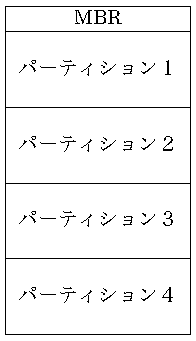
\includegraphics[scale=0.8]{../Fig/hddPartition.pdf}}
    \end{minipage}
    \begin{minipage}{0.3\columnwidth}
      \centering{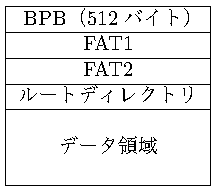
\includegraphics[scale=0.8]{../Fig/fatVolume.pdf}}
    \end{minipage}
    \begin{minipage}{0.3\columnwidth}
      \centering{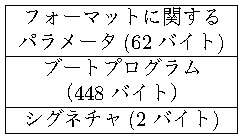
\includegraphics[scale=0.8]{../Fig/fatBPB.pdf}}
    \end{minipage}
  }
  \vfill
  \begin{itemize}
  \item (ディスク装置全体,または,パーティション) = ボリューム
  \item パーティションの位置と大きさはMBRのテーブルで決まった.
  \item ボリュームの内部構造はFATファイルシステムのルールで決まる.
  \item ボリューム内部のコンポーネントの大きさなどはBPBから分かる.
  \item FATは大切なデータなので2重化してある.
  \item データ領域は\emph{クラスタ}と呼ばれるブロック単位で扱う.
  \end{itemize}
  \vfill
\end{frame}

%=========================================================================
\begin{frame}
  \frametitle{BPB(BIOS Parameter Block)}
  \tbl{scale=0.9}{fatBpbParameter.pdf}
  \begin{itemize}
  \item 論理フォーマット時に決めたパラメータを記録している.
  \item 値の例は,ボリューム=2GiB,クラスタ=32KiB,FAT16
  \item ブートプログラムは初代IBM PCの機械語で作成してある.
  \end{itemize}
  \vfill
\end{frame}

%=========================================================================
\begin{frame}
  \frametitle{ディレクトリエントリ}
  \fig{scale=1.0}{fatDirEntry.pdf}
  \begin{itemize}
  \item ルートディレクトリやディレクトリファイルに格納される.
  \item 前のBPBだとルートディレクトリに512個格納される.
  \item \texttt{FileName}:8文字以内のファイル名\\
    (0x00:以降未使用,0xe5:削除,0x05:本当は0xe5)
  \item \texttt{Ext}:3文字以内の拡張子
  \item \texttt{Atr}:ファイルの属性\\
    (0x01:read-only,0x02:hidden,0x10:dirextory...)
  \item \texttt{Time}:ファイルの最終変更時刻
  \item \texttt{Date}:ファイルの最終変更日
  \item \texttt{Cls}:データが格納されている先頭クラスタの番号
  \item \texttt{Size}:ファイルの大きさ(バイト単位)
  \end{itemize}
\end{frame}

%=========================================================================
\begin{frame}
  \frametitle{FAT(File Allocation Table)}
  \centering{
    \begin{minipage}{0.45\columnwidth}
      \centering{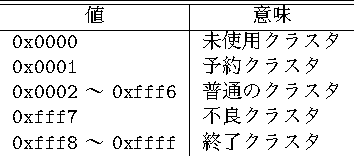
\includegraphics[scale=0.9]{../Tbl/fatClsNum.pdf}}
    \end{minipage}
    \begin{minipage}{0.45\columnwidth}
      \centering{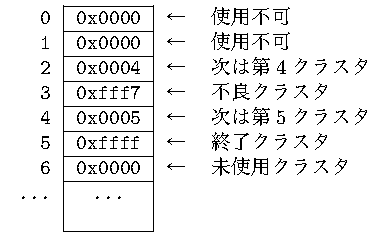
\includegraphics[scale=0.9]{../Fig/fatConcept.pdf}}
    \end{minipage}
  }
  \vfill
  \begin{itemize}
  \item クラスタをファイルに割り当てる表
  \item FATエントリとクラスタが一対一対応
  \item FAT16ではFATエントリが16ビット
  \item \texttt{0x0002}〜\texttt{0xfff6}が普通のクラスタ番号
  \item \emph{クラスタチェイン}を形成する.
  \item ディレクトリエントリの\texttt{Cls}がチェインの先頭を指す.
  \end{itemize}
\end{frame}

%=========================================================================
\begin{frame}
  \frametitle{FATファイルシステムの全体像を示す例}
  \fig{scale=0.7}{fatFileSystem-crop.pdf}
\end{frame}

%=========================================================================
\begin{frame}
  \frametitle{ディレクトリファイル}
  \lst{numbers=none}{fatDirDump.txt}
  \begin{itemize}
  \item ルートディレクトリ以外のディレクトリは\texttt{Atr=0x80}のファイル
  \item リストはmacOSでFAT16ファイルシステム上で実験した例
  \item 最初の2エントリーは\texttt{.}と\texttt{..}を格納している.
  \end{itemize}
  \vfill
\end{frame}

%=========================================================================
\begin{frame}
  \frametitle{練習問題}
  \begin{enumerate}
  \item[1.] 次の言葉の意味を説明しなさい.
    \begin{itemize}
    \item BPB
    \item ルートディレクトリ
    \item クラスタ
    \item ディレクトリエントリ
    \item FAT
    \item クラスタチェイン
    \item ディレクトリファイル
    \end{itemize}

  \item[2.] ディレクトリファイルのダンプリストを
    ディレクトリエントリの構造と比較しながら解析しなさい.

  \item[3.] 全体像を示す例の\texttt{ABCDEFGH.TXT}ファイルの
    第\texttt{0x00002000}バイトが格納されるクラスタの番号を答えなさい.

  \item[4.] 前問と同様に,
    第\texttt{0x00004000},\texttt{0x00008000},\texttt{0x00010000}
    バイトに付いて答えなさい.
  \end{enumerate}
\end{frame}

%=========================================================================
%\begin{frame}
%  \frametitle{}
%\end{frame}

\end{document}
